\documentclass{article}

% Language setting
% Replace `english' with e.g. `spanish' to change the document language
\usepackage[english]{babel}

% Set page size and margins
% Replace `letterpaper' with `a4paper' for UK/EU standard size
\usepackage[letterpaper,top=2cm,bottom=2cm,left=3cm,right=3cm,marginparwidth=1.75cm]{geometry}

% Useful packages
\usepackage{amsmath}
\usepackage{indentfirst}
\usepackage{graphicx}
\usepackage{subcaption}
\usepackage{float}
\usepackage[colorlinks=true, allcolors=blue]{hyperref}

\title{Parameter Packing: Automated Notification of Refactoring for Readability}
\author{Jarred Bettencourt, John Broderick, Bryan McCaffery, Joseph Black}

\begin{document}
\maketitle 

\begin{abstract}
With software and technology becoming so core to the lives of billions over the world, it becomes increasingly important to have intuitive and informative analytics about codebases that we develop and use. This becomes especially true with codebases that evolve to become monolithic and have potentially thousands of developers, like common open open source projects. Without stressing nonfunctional requirements like readability, development organizations risk losing many hours familiarizing new developers with code which is time that could be spent developing new features or debugging. To allow developers to make more informed decisions, we present Parameter Packing, which is a toolchain to alert developers to code that could be made more reusable with slight changes. More specifically, our module notifies developers that multiple parameters could be combined into an object when they are commonly shared across several functions in a codebase, which alleviates developers from the extraneous task of remembering parameter orders, or constantly specifying unique parameters. Our results show that with files in popular open source projects, our developed algorithms are able to very easily alert developers to possible packings with extremely low overhead for medium to large files.  
\end{abstract}

\section{Introduction}

The massive scale of modern software and its widespread integration into our daily lives continues to impact billions around the world with respect to every facet of human life. Whether it be the way that we communicate with each other, or the way that we entertain ourselves, it is difficult to find an activity that has not been wholly transformed by the introduction of software.

Still, this monolithic scale and our ever-growing dependence on software introduces challenges implicit to complex codebases in any form. A pertinent issue that comes as a consequence of these problems is system maintenance and maintainability. As human interest changes, it is important to be able to easily modify software in order to better suit the needs of users which becomes exponentially more difficult if a particular codebase is not standardized or readable. Additionally, with lower standardization and readability among files in the same codebase, developer time is wasted on trying to understand extraneous program details when time would be better spent improving functionality or efficiency of a program.

In the attempt to remedy this, we have developed a tool for ``parameter packing". Parameter packing is our term for taking different methods, comparing their parameters, and notifying the programmer that placing redundant parameters from separate methods into an object that can be passed to the methods could simplify program design from a readability perspective. An example could be the following:

\begin{itemize}
    \item Suppose we have method 1 with input parameters A, B, C, and G.
    \item Suppose we have method 2 with input parameters A, B, C, D, E, F.
    \item The parameter packing algorithm would notify the programmer that
    \begin{itemize}
        \item Method 1 with input parameters Object parameter $\alpha$, and Variable parameter G.
        \item Method 2 with input parameters Object parameter $\alpha$ and Variable parameters D, E, F.
        \item Object parameter $\alpha$ would be defined as holding the information for Variable parameters A, B, C.
    \end{itemize}
\end{itemize}
This removes the need for methods that contain a large amount of parameters, and we believe can help to increase the readability and standardization of the code. With a higher degree of standardization and readability, it it reasonable to assume that developers will have an easier experience learning a codebase when first starting to develop for said codebase. We believe giving users increased insight into their codebase will allow for a higher degree of accessibility with respect to new developers joining a project after development has begun.


\section{Prior Work}
\begin{enumerate}
    

    \item \textbf{Improving Code Readability Models with Textual Features:} The authors Scalabrino et al.\cite{7503707} want to expand what readability models consider when classifying code as either readable or unreadable. Prior to their work, the authors lament that readability models only consider structural aspects of code such as line lengths and comments. Scalabrino et al. Present textual features that can measure code readability in terms of source code lexicon. Using over 5k people to manually review 600 code snippets and rank their readability, the authors proceed to compare ML models that use their textual features versus conventional models that use structural features. The authors confirm that their textual features can be combined with the prior structural features to improve the accuracy of readability models significantly. The main focus of this paper is on automatically determining readability of code using an ML model; our research is also attempting to automate a normally manual and labor-intensive task. Where our research differs from Scalabrino et al. is that their focus is on code readability detection, ours is on automatic mutation / refactoring to improve readability. A more specific difference is that their research is using a statistical ML model versus our approach which will likely be more algorithmic in nature.

    \item \textbf{Code Readability Testing, an Empirical Study:} The goal of Sedano’s research is to develop a technique called Code Readability Testing thats usable as a metric for determining the readability of code. He also seeks to determine whether or not the technique improves participating programmers’ ability to write code that’s readable. The author proceeded to have 21 programmers follow his Code Readability Testing technique over 4 sessions. In brief, the methodology of these sessions is that an author of code is paired with a reader who reviews the codebase. The session begins with author describes the use case or functionality of some code and goes over the modified files; the reader then proceeds to read aloud the codebase, speculating outloud about unclear sections, and explaining how the reader thinks it works. During this time, the author takes notes on what is confusing, and afterwards the author clarifies any issues the reader expressed and then they jointly discuss how to improve the readability of the code. As a result, 16 of the 21 participants showed some improvement in their ability to write readable code. The main takeaways that are relevant to our research is twofold: there is an unnecessary time cost associated with reviewing unreadable code, and we conjecture that for expanding such a codebase, this time cost balloons; writing readable code cuts this time-cost significantly. Secondly, the paper provides data on the most-common ways to improve the readability of their code. The most common were things like improving variable and method names, simplifying the conditions of branches and loops, and removing code duplication with more methods. What’s interesting, is that they didn’t really discuss any forms of parameter adjustment, with only 1 note about “re-sequencing method arguments”\cite{7474473} in their data. Our research wants to avoid manual revision and rely on an automated procedure to save time, and our focus is on object packing to reduce parameter bloat of functions. 

    \item \textbf{Identification of Extract Method Refactoring Opportunities:} This paper addresses the research question of which approaches can decompose a method into sub-methods, i.e. perform the "Extract Method"\cite{4812745} refactoring. The authors outline approaches involving slices of the program, which divide the control flow graph into blocks which are suitable for separation into discrete methods. This paper answers a different research question than ours because it is instead focused on the Extract Method refactoring. That said, its automated refactoring methods may provide relevant background as we seek to apply our own static transformations to the method structure of a program.

    \item \textbf{Identifying, Tailoring, and Suggesting Form Template Method Refactoring Opportunities with Program Dependence Graph:} This paper\cite{6178876} researches an automated method for refactoring to remove code clones using the Form Template Method refactoring. Code clones are duplicate (or near-duplicate) sections of logic that can be eliminated with the process of inserting a template method that allows similar variations of the process to run. This approach works by identifying subsets of nodes within the Program Dependence Graph. Our own research questions do not focus on application logic. However, our goal of replacing duplicate or near-duplicate function signatures with a more compact replacement is conceptually very similar to the approach undertaken in this paper. We may adapt algorithms proposed here for our own purposes.
  % END Joseph's summaries.
  \item \textbf{An Empirical Study on API Parameter Rules:} This paper\cite{10.1145/3377811.3380922} investigates the general concept of parameter ``rules" in software. In this context, a parameter rule is a certain methodology of parameters in a function/method which are consistent among the entire program. For example, a parameter rule could be to avoid optional values in an entire codebase, or to use default values at all possible points. This paper sets out to manually find parameter rules within software (denoted as PaRu), and detail their consistency among all software developers in their sample. The findings suggest that a large portion of developers, whether consciously or unconsciously, utilize similar parameter rules when developing software when developing in a collaborative setting. Our project aims to find ways in which to alter parameters of methods/functions to successfully improve readability, and this paper is studying how consistent parameter rules are between codebases. It may be useful to analyze this paper, and determine which parameter rules our project should try to place on a codebases during refactoring to remain consistent among developers and other teams.
  \item \textbf{A New Algorithmic Approach to Finding Minimum Spanning Tree:} With their paper detailing the minimum spanning tree problem and its implications for computer science, Khan et al.\cite{inproceedings} additionally discuss a new algorithmic approach that more efficiently finds an MST of a set than the cutting edge algorithm at the time. The algorithm heavily leans on the disjoint set union data structure on computers for its implementation. At the time of publication, this usage of set operations to find an MST was not heavily studied, and this paper presents a novel approach for finding an MST with the usage of a data structure (such as something that would be found on Java). In our project proposal, we plan to investigate the possibility of looking at parameters in a function or method as a set, and creating an MST to determine which functions should have their parameters packed into objects to increase readability. A consistent usage of an MST on a codebase through our refactoring program will allow parameters in functions/methods to potentially be more consistent with other methods/functions defined in the same codebase. This paper provides a method to find an MST effectively, which we may use for our purposes.
\end{enumerate}

\section{Basis for Our Method}

The existing work we surveyed for automatic refactoring approaches follows a process of constructing a data structure from the input source code and then performing transformations on it. For example, \cite{4812745} performs the Extract Method refactoring by operating on a program dependence graph. Our problem of parameter packing does not require dependence information though, or in fact knowledge of application logic at all. So we can produce a more minimal structure which just focuses on the function signature.

Graph structures such as the one from \cite{10.1145/3377811.3380922} define nodes and edges, respectively, based on atomic components of the program structure and the relevant relationship between them. A key property we set out to analyze is the number of shared function signatures between two parameters. This metric defined for a pair of nodes in a graph lends itself naturally to a weighted undirected edge.

\section{Toolchain Architecture}

\noindent Our toolchain is implemented in Python, along with a handful of helper shell scripts and a Makefile. The Makefile and shell scripts jump-start the toolchain, along with handling both building and cleaning up dependencies. Once the Makefile is invoked with the \textit{run} target, the input file will enter our pipeline.
\newline\newline
\noindent\textbf{Architecture Pipeline}
\begin{enumerate}
    \item Preprocessing:  Does necessary modifications prior to processing
    \item Frontend: Collects function signatures
    \item Packer: Packs parameters and updates function signatures
    \item Visualization: Provides suggestions for parameter packings
\end{enumerate}

\noindent All components but Preprocessing are modular --- when the toolchain is invoked, the user specifies a frontend, packer, and visualizer to use. We have written one implementation for each component, which will be described in further detail below. A determined user could feasibly write their own components with little to no modifications to the existing codebase. 

Modules are invoked in the format \textit{file\_name.ClassName}; an example invocation of our toolchain on file \textit{foo.c} is shown below:
\begin{verbatim}
    make run FRONTEND=source_parser.SourceParser \
    PACKER=aggressive_minimize.AggressiveMinimize \
    VISUALIZER=html_visualizer.HTMLVisualizer FILE=foo.c
\end{verbatim}

\noindent This will run the toolchain using our team's implementations of each component. All modules assigned here are optional, but they will be replaced with a default module with minimal functionality.

All software and reports can be found in our repository, located on \href{https://github.com/jbettencourt10/parameter-packing-621}{Github}.


\subsection{Preprocessing}

\noindent Unlike all other components of our pipeline, the Preprocessing component is not handled by the Python runner, and is instead a simple shell script called \textit{remove\_comments.sh} that is invoked by \textit{run.sh} prior to executing the python runner.

Those who wish to extend the functionality of the Frontend for the purposes of supporting other languages or other methods of function signature extraction will likely have to remove or replace this component in the pipeline.

The functionality of our Preprocessor is trivial --- the input file has comments stripped by running it through gcc preprocessing; the output of this step creates a file with the same filename but appended with the additonal extension ".nocomments". For example, when run on \textit{test.c}, the Preprocessor script will output \textit{test.c.nocomments}, which the toolchain uses for the remainder of the pipeline. See Figure \ref{fig:preprocess_example}.

\begin{figure}[ht]
    \subcaptionbox*{test.c}[.45\linewidth]{%
        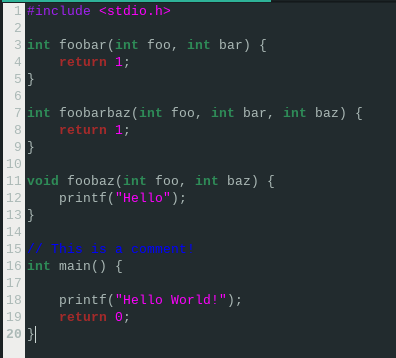
\includegraphics[width=\linewidth]{im1.png}%
      }%
      \hfill
      \subcaptionbox*{test.c.nocomments}[.45\linewidth]{%
        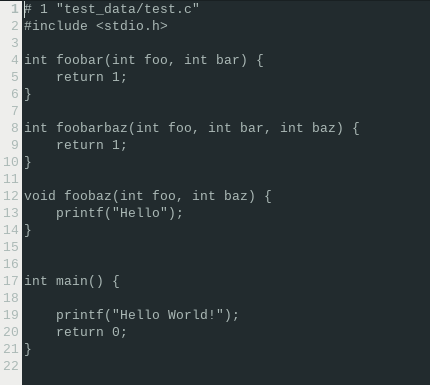
\includegraphics[width=\linewidth]{im2.png}%
      }
      \caption{Preprocessing Example}
      \label{fig:preprocess_example}
\end{figure}

\subsection{Frontend}

\noindent The Frontend is what extracts function signatures from a file, and converts the resulting information to our intermediate JSON format with the name \textit{FILENAME.json} (more on this in \ref{intermediate_json}). Our toolchain expects a valid Frontend module to implement a class that takes a filename and the maximum number of parameters in a function, as input. There must be a class function parse() with no parameters, which will produce the JSON output for the rest of the pipeline. See Figure \ref{fig:frontend}.
\newline\newline

The relevant information to be captured about the source code is contained in the signature of each function declaration. The graph representation used by parameter packing algorithms needs a list of all the parameters for each function name.

To handle the full range of possible valid input files, a parser would need to be constructed or adapted to extract these components from the source code. However, for the purposes of demonstrating and evaluating our methods on real data, a simpler process can be used. We define a regular expression for matching function signatures, and further specify the capture pattern that will extract the function name and parameters. Longstanding methods stemming from \cite{10.1145/363347.363387} for this computation have been implemented in standard libraries for many languages, such as Python in our case.

The output from this stage is then, abstractly, a mapping $F \to \{ p_1, p_2, ..., p_n \}$ from the function name to the set of that function's parameters. We implement this as a two dimensional list which is then serialized to JSON for processing by the subsequent stages.

A benefit of this method is that the layout of the regular expression allows researchers to work with a direct symbolic definition of the defined pattern to match for capturing relevant components of function signatures. Unfortunately, because the full function signature might have a variable number of parameters, only up to a maximum user-specified number of parameters can be retrieved. This maximum value defaults to 10. See the Future Work section for a discussion of improvements to this.

\begin{figure}[ht]
    \subcaptionbox*{test.c.comments}[.45\linewidth]{%
        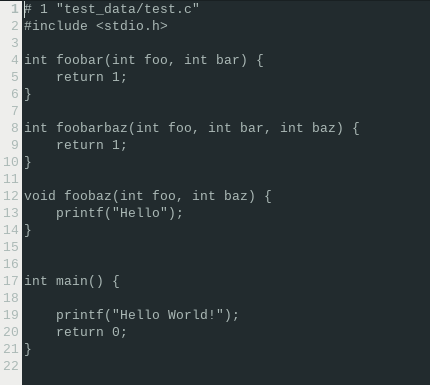
\includegraphics[width=\linewidth]{im2.png}%
      }%
      \hfill
      \subcaptionbox*{test.json}[.45\linewidth]{%
        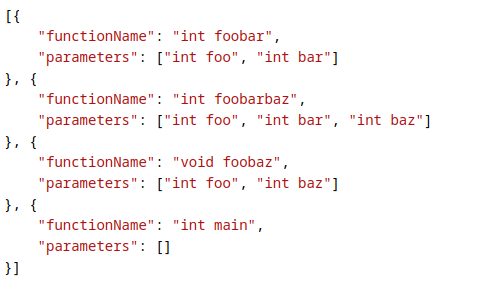
\includegraphics[width=\linewidth]{im3.png}%
      }
      \caption{Frontend Input and Output}
      \label{fig:frontend}
\end{figure}

\subsection{Intermediate JSON format} \label{intermediate_json}

To adequately link together the frontend portion of our project which parses files with the backend which consists of attempting to find an optimal way to pack parameters, it is necessary to include an intermediate representation that can be output by the frontend and input to the backend. Additionally, it is necessary to have an intermediate representation for the output of the packing backend to input into our visualization stage which helps to notify programmers of the structure of their program. We accomplish this using JSON as our intermediate representation, which is easily and efficiently parsed at all steps of our pipeline. 

Due to the existence of two phases where it is necessary to have JSON represent the state of a parsed file, we have created two separate JSON representations. The first representation is for the integration phase between our frontend/regex and our packing algorithm. As shown in figure \ref{fig:frontend}, the format of JSON for this phase is the following,

\begin{verbatim}
    [{
    "functionName": "returnType functionName",
    "parameters": ["parameterType parameterName", "..."]
    },
    ]
\end{verbatim}

which allows for an intuitive parsing to the backend. This JSON representation is then transformed into a custom built class used for a graph representation (allowing us to find parameter packings), where each node of said graph is a parameter, and the edge weight between two parameters is the number of functions where both parameters exist as an argument. 

The second phase that requires a JSON representation is a representation that will be used for the output of the packing algorithm to allow visualization and notifying the programmer of possible packings. With this particular representation, it is possible to parse the output of potential packed parameters and display to the user in an HTML file. The intermediate representation for JSON in this section has the following format

\begin{verbatim}
    [{
    "packed_param": "newParameter",
    "parameters": ["parameterType parameterName", "..."]
    },
    ]
\end{verbatim}

This format is used to tell the user that the parameters specified in the above parameters list are commonly shared and can be packed together into newObject to allow for the reuse of variables throughout the lifespan of the codebase and program. Using a graph visualization and a detailed list, information is shown to the user in an intuitive way to allow for action to be taken to increase readability.

\subsection{Packing Algorithms}

\noindent The packer component is responsible (as the name suggests) for finding duplicate parameters in function signatures, and packing them together (In the case of C, as structs). A valid packer module must define a class that takes a filename as input (a JSON file produced by the Frontend component), and it must have a class function minimize() that has no parameters, and produces two JSON files as output; these output files are called \textit{FILENAME\_updated.json}, which stores the updated function signatures that now include packed parameters, and \textit{FILENAME\_packed.json}, which stores what parameters are packed into each packer parameter. See Figure \ref{fig:packer_example}.

We have implemented three (albeit similar) packing modules --- Aggressive Minimize, Percentage Minimize, and Weighted Percentage Minimize. A user who wishes to create their own packer module could do so with no modification to the toolchain, assuming they follow the specification outlined above.

Our modules are best explained with a graph analogy; every parameter is a vertex, and every edge means that both parameters appear together in a function signature. Every edge has a cost, and every time both parameters are in a function signature together, the cost is incremented. The algorithms then reduce this graph, by combining nodes in a way specified by the different algorithms. This approach mirrors \cite{6178876} which searches and combines nodes in the program graph.

\subsubsection{Aggressive Minimize}

\noindent  

In Aggressive Minimize, parameters are combined based on the highest available edge weight. If there exists an edge with cost greater than 1 (the pair appears in at least two functions), then the edge with the greatest cost will have their vertexes combined. See Figure \ref{fig:agmin_example}. Function signatures are updated with this new packed parameter, and edges are rebuilt. This process will continue until all remaining edges have a cost of 1 (or no edges remain).

Our module begins at class instantiation, where the JSON function signatures are extracted from the input file, and Python Function and Parameter class objects are created. When minimize() is called, the algorithm will use the list of Function objects to follow the above algorithm: build edges, combine vertexes with heaviest edge, repeat until end condition is reached. At the conclusion of this, the now-modified list of Functions is converted into JSON and the packed parameters are also converted to JSON.

The general effect of this algorithm is that packed objects bubble together. There are no nested packed parameters, so if two packed parameters share a parameter, they are combined (via set union) into a new packed parameter. This can result in larger than desired packed objects, depending on how parameters are shared.

\begin{figure}[ht]
    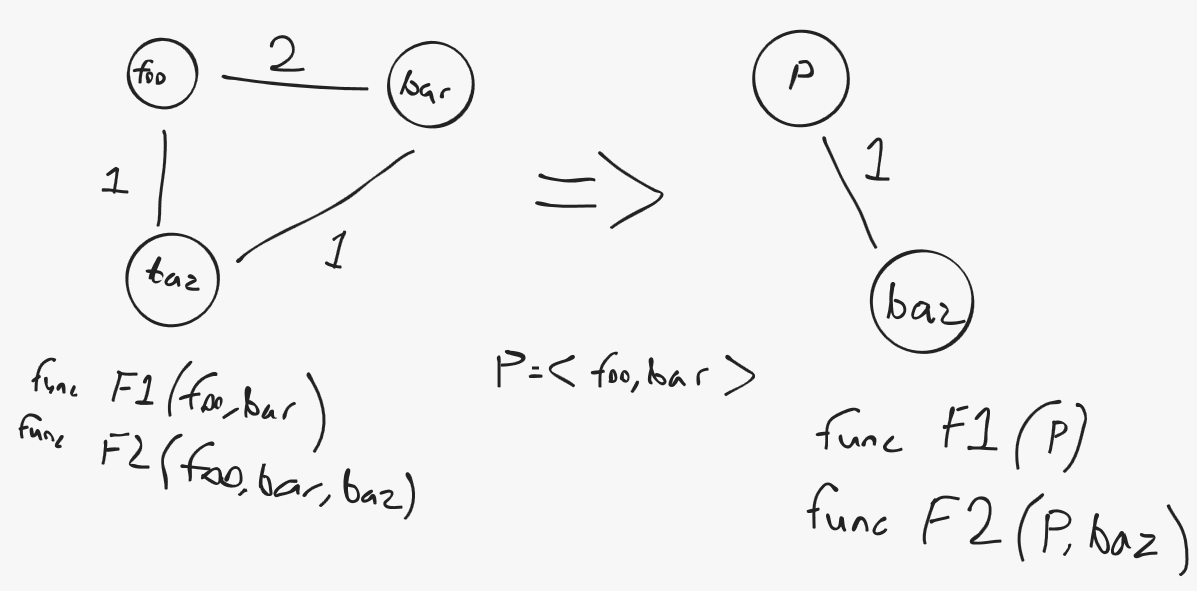
\includegraphics[width=\linewidth]{im7.png}
    \caption{Aggressive Minimize Vertex Combination Example}
    \label{fig:agmin_example}
\end{figure}


\subsubsection{Percentage Minimize}

In percentage minimization, the algorithm combines the two nodes that have an edge weight that has the highest percentage of the total edge weight for the two nodes. This uses the average of the percentage the edge is for each respective node. The percentage edge weight is calculated for every edge, then the nodes of the largest percentage edge are combined into a single packed node. The graph is then recalculated with this packed node, and the process is repeated until all edge weights are equal to one.

The goal of this algorithm is to find parameters that are most commonly together, without factoring in the number of occurrences. This means two parameters that only appear together, but are only in one function together will be packed, before two parameters that appear a million times, but are only together half the time. The packed objects cannot have a packed object inside of it, and packed objects are combined via union. There is no minimum requirement for parameters to be packed, as such the packed parameter objects can result in larger than desired objects. 


\subsubsection{Weighted Percentage Minimize}
In weighted percentage minimization, the algorithm calculates a new edge weight for each of the edges. This new edge weight calculated by taking the percentage of the total edge weight for each of the respective nodes, averages the percentage, and multiplies the average percentage by the edge weight. The edge with the largest new calculated weight, has its two nodes combined, and then the graph is recalculated with the new edge, and is repeated until each of the edge weights are either zero or one.

The goal of this algorithm is to find parameters that are most commonly together, while factoring in the number of occurrences. The number of occurrences is weighted by the percentage, as such two parameters that share five functions and only appear together with no other parameters will be packed after two parameters that appear together a million times, but only ten percent of their occurrences are together. However the main benefit of this algorithm is the cases where edge weights are similar. In the case of two sets of two parameters where both occur together the same amount of times, the algorithm will combine the set of nodes where they are shared by fewer parameters first.

\begin{figure}[ht]
    
    \subcaptionbox*{test.json}[.3\linewidth]{%
        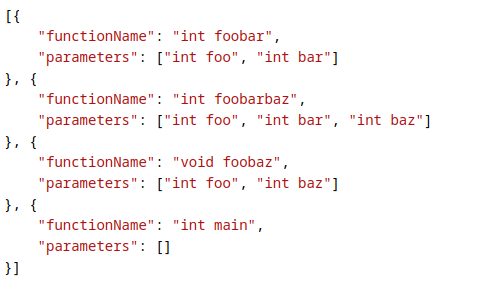
\includegraphics[width=\linewidth]{im3.png}%
      }
    \hfill
    \subcaptionbox*{test\_updated.json}[.3\linewidth]{%
        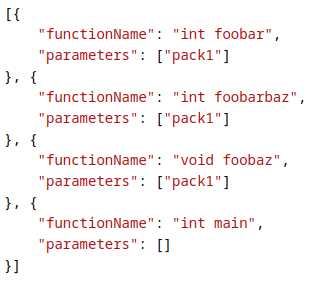
\includegraphics[width=\linewidth]{im4.png}%
      }%
      \hfill
      \subcaptionbox*{test\_packed.json}[.3\linewidth]{%
        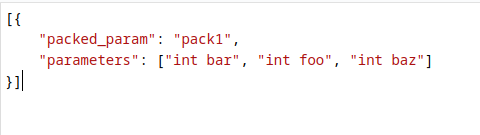
\includegraphics[width=\linewidth]{im5.png}%
      }
      \caption{Packing Example - using the Aggressive Minimize algorithm}
      \label{fig:packer_example}
\end{figure}


\subsection{Visualization}

\noindent Visualization modules provide suggestions for how to pack parameters. Our module presents this in the form of a report in HTML. 

In order for a Visualization module to be up to spec, the class must take a filename as input; this filename is \textit{filename.json}, output by the frontend. The module class must have a function visualize() with no parameters, which will produce the final output of the toolchain. See Figure \ref{fig:visual_example}.

The output of the packer is a two json files. The visualizer turns the json output into a series of suggested objects for packing parameters. 
The visualizer shows the parameter maps, original parameters, and our tools suggestion for packing. The parameter maps, are graphs where each node is a parameter, and the edges are how many functions share the two nodes. These graphs offer a visual representation of how often parameters are shared between functions. The original parameter list is included to show the reduction.

The main piece of information is the suggested packing list. For each object in the packing list there are two major pieces of information. The first is the parameters that will be in each of the objects. Each parameter can only be in one object, and except in rare cases all items in the original parameters will be in a packed object. The second piece of information is the functions that will use the suggested parameter packing. This list of functions is all of the places the developer would need to update the code in order to use our packed parameter object. Finally there is also a name assigned to our object, as well as the number of occurrences to allow for easy consideration. 

\begin{figure}[ht]
    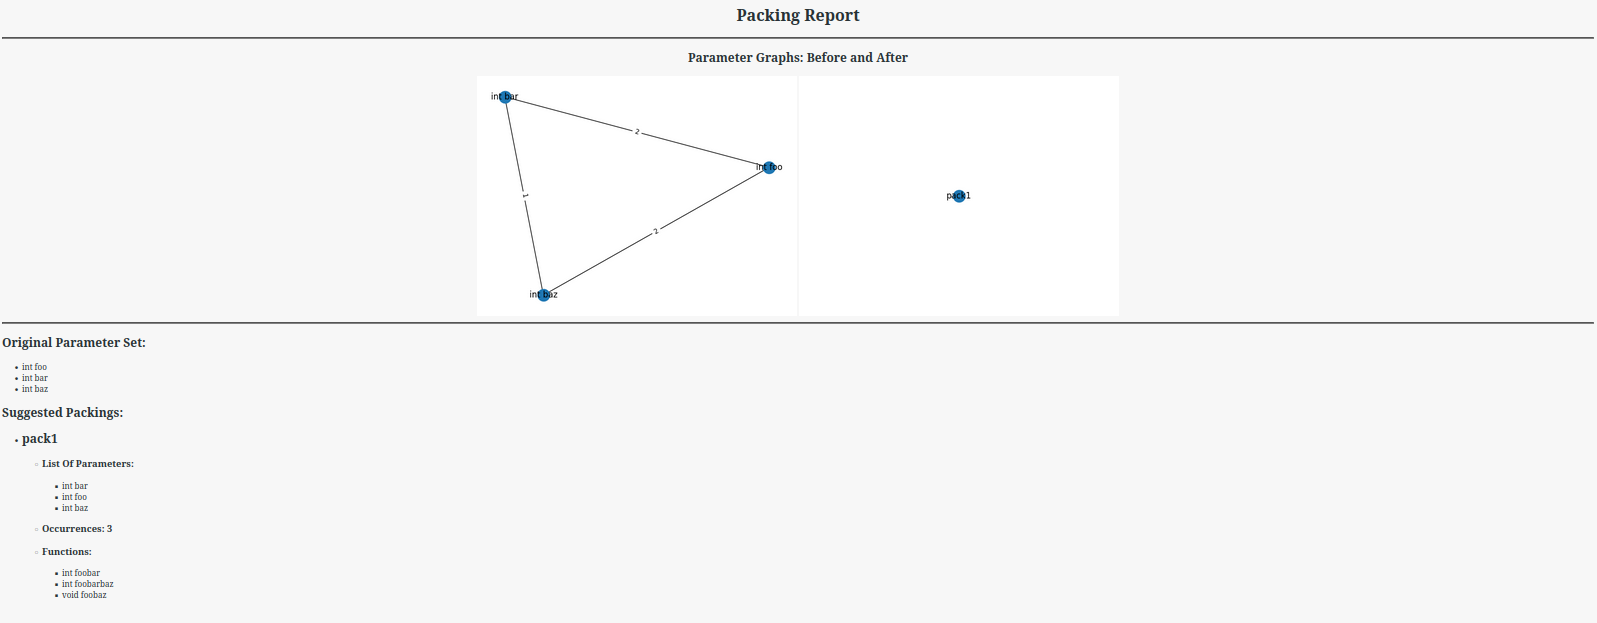
\includegraphics[width=\linewidth]{im6.png}%
    \caption{Visualization Example}
    \label{fig:visual_example}
\end{figure}

\newpage

\section{Results}

We chose several open-source repositories written in C or C++ from GitHub as a method of testing the refactoring capability of our tool. Our list for evaluation of the tool is composed of the following projects:

\begin{enumerate}
    \item OpenSCAD: a software for creating solid 3D CAD objects.
    \item GIMP: a GNU image manipulation program.
    \item Libreoffice: an integrated open source office suite.
    \item qBittorrent: a BitTorrent client for P2P connections.
    \item PCSX2: a free and open-source PlayStation 2 (PS2) emulator.
\end{enumerate}

We believed that testing the ability to pack parameters in these projects ensures that our tool is versatile in C/C++ projects of any use. Additionally, using our project with such a large breadth of repositories means there is a high likelihood of the reusing of parameters, making our tool useful. 

The algorithms reduce the parameters to packed parameters if there are multiple occurrences where parameters are shared. The results offered by the different algorithms are the same in many cases. For the weighted percentage and aggressive minimize algorithms, the outputs were the same for all examples from open source projects. There are cases where the results differ, but it requires specific conditions to be met which did not appear in any of the open source projects. In a program purposely written to show the differences, the results were still very similar. Percentage minimize on the other hand, offers differing results on many of the example programs.


\subsection{PCSX2}

As an example from PCSX2, we took Host.cc, which has a variety of parameters and functions where many of them are shared. The results of all three packing algorithms were equivalent, creating one packed object, used by 23 different functions. This reduced the number of parameters from 15 to 7, a reduction of roughly 50\%. See Figure \ref{fig:pcsx2_graph}.


\begin{figure}[ht]
    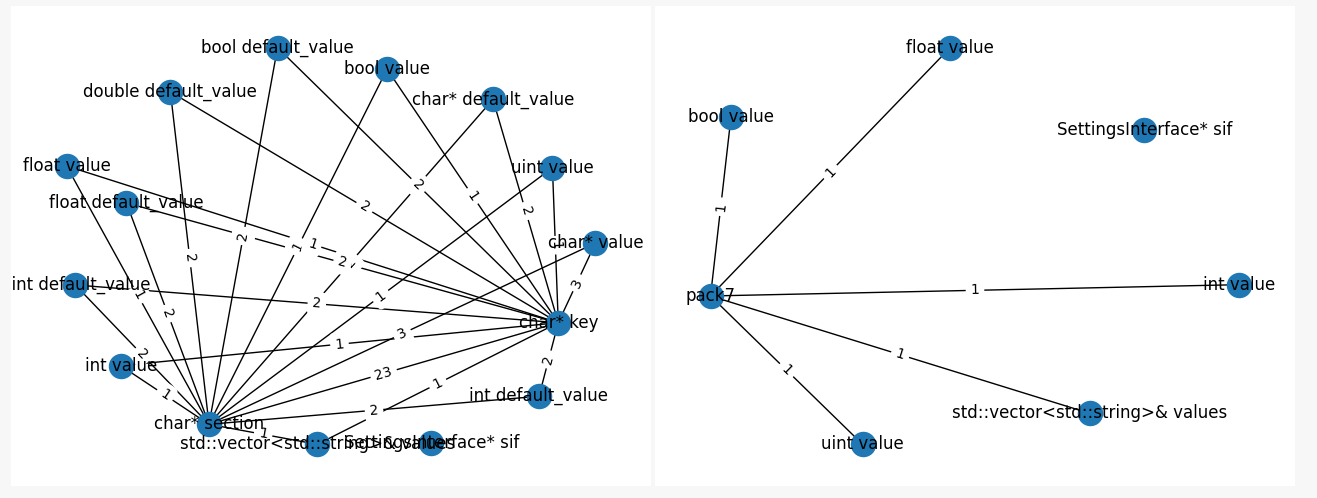
\includegraphics[width=\linewidth]{im8.png}%
    \caption{Before and after packing Host.cc from pcsx2}
    \label{fig:pcsx2_graph}
\end{figure}


\subsection{Libreoffice}

\begin{figure}[ht]
    \subcaptionbox*{Original}[.3\linewidth]{%
        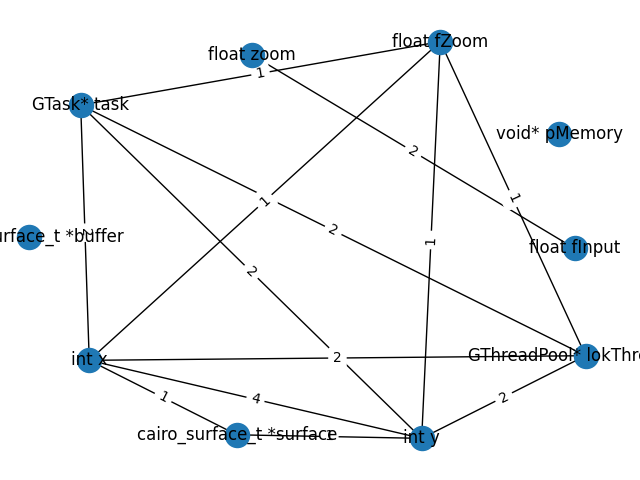
\includegraphics[width=\linewidth]{tilebuffer_original.png}%
      }
    \hfill
    \subcaptionbox*{Aggressive Minimize}[.3\linewidth]{%
        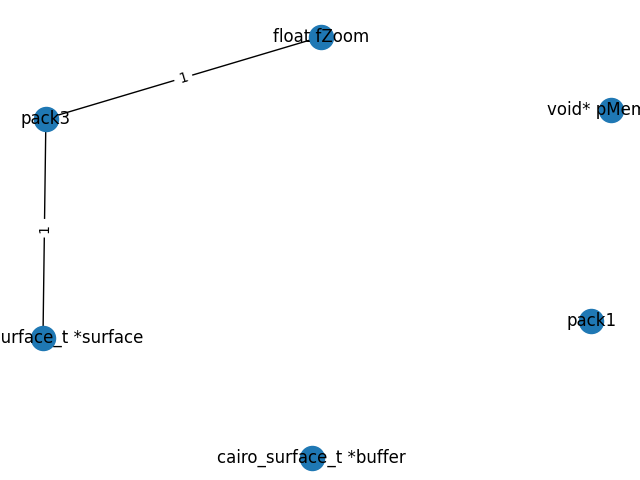
\includegraphics[width=\linewidth]{libreoffice_a.png}%
      }%
      \hfill
      \subcaptionbox*{Percentage Minimize}[.3\linewidth]{%
        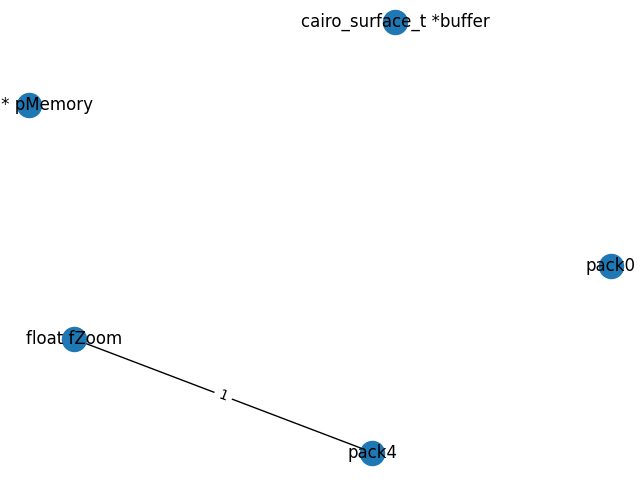
\includegraphics[width=\linewidth]{libreoffice_p.png}%
      }
      \caption{Libre Office Parameter Packing}
      \label{fig:libreoffice_example}
\end{figure}

The results given by the aggressive minimize and percentage weight minimize are the same for the example from libreoffice. However the result for percentage gives a different result. This is due to the fact that the percentage will combine nodes that have an edge with a weight of one, if there are other edges that are still greater than one. It also chooses nodes to combine in a different order. This creates a situation as seen where a packing is made that would not be done in the other algorithms and the differing results. See Figure \ref{fig:libreoffice_example}.


\section{Conclusion}
We believe that incorporating our parameter packing toolchain into a development project has the potential to give developers further insight into the code they are developing on a scale larger than the file they are currently editing. With increased information about code that one is writing and code that is being written by other members of an organization, it becomes much easier to get acclimated to a new codebase. This ease of acclimation means that developers will not have to spend time concerning themselves with unimportant details like parameter orders or the repeated specification of parameters for different function calls. With this newfound time, developers will have more time focusing on aspects like new functionality.  In general, we believe automating the workload of developers allows for the reallocation of time to more important aspects of software development, and we have found that in popular open source projects, our toolchain is successful in automating tasks for developers in an effective and efficient manner.

\section{Future Work}
\subsection{Frontend}

While a regex can be used in most cases to parse function signatures, it can be finicky, resulting in unexpected outputs; a better solution is to use a C parser that understands the grammar of the C language, which should result in more accurate outputs. In addition, our experiments also show that evaluating the regular expression on a large file can take several seconds even on a modern desktop CPU. Additional investigation would be needed to establish conclusively that a parser would operate more quickly.

\subsection{Reconstruction}
The likely progression of this tool is the reconstruction of code bases using the results of our parameter packing. This does not require any further research, it only requires development time. In the current implementations of our algorithms, it is the case of finding all instances of a variable that has been packed and replacing it with an object that represents the packed parameter. This requires many considerations of pointers, arrays, and other conversion cases, and as such was out of scope. 
\subsection{Visualization}
One area of future work is a better visualization tool. The current visualization tool only shows one algorithm's results. A better tool would allow for the developer to swap between results of the different algorithms, and allow them to easily analyze the results of the different algorithms from a single screen. Another advancement would be the launching of the reconstruction from the visualization. Allowing the workflow to be run the tool, analysis, choosing a result, and then reconstruction of the program with the packed parameters to be done from a single interface.
\subsection{Algorithms}
Another area of future research is in regards to better algorithms to pack the parameters. As the goal is readability, there is no optimal solution as readability is not a discrete value.The algorithms in our paper only do calculations in regards to the number of times it occurs in functions with other parameters. This offers a single data source to make considerations on when to pack it with another parameter, and does not consider other data that may be useful such as the number of parameters in a function. The algorithms also do not consider how many parameters are in an object which leads to large packed parameters. This leaves room to develop improved algorithms in future work. 

\bibliographystyle{alpha}
\bibliography{sample}


\end{document}